\begin{exercice*}
    Toutes les rotations sont à effectuer dans le sens anti-horaire.
    \begin{enumerate}
        \item Construire $C$, l'image de $B$ par la rotation de centre $A$ et d'angle \ang{90}.\\
        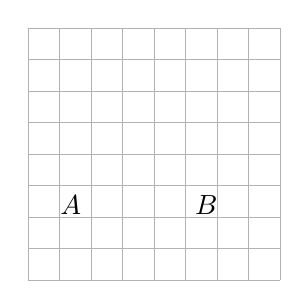
\begin{tikzpicture}[scale = 0.4]
            \draw[help lines, color=black!30] (0,0) grid (8,8);        
            \coordinate[label=below left:$A$] (A) at (2,3);
            \coordinate[label=below right:$B$] (B) at (5,3);
            \tkzDrawPoints[shape=cross out,size=3pt](A,B);
        \end{tikzpicture}
        \item Construire $F$, l'image de $E$ par la rotation de centre $D$ et d'angle \ang{90}.\\
        \begin{tikzpicture}[scale = 0.4]
            \foreach \x in {0,1,...,8} {
                \foreach \y in {0,1,...,8} {
                    \fill[color=black] (\x,\y) circle (0.05);
                }
            }
            \coordinate[label=above left:$E$] (E) at (3,7);
            \coordinate[label=above right:$D$] (D) at (5,4);
            \tkzDrawPoints[shape=cross out,size=3pt](E,D);
        \end{tikzpicture}
        \item Construire $K$, l'image de $H$ par la rotation de centre $G$ et d'angle \ang{60}.\\
        \begin{tikzpicture}[scale=0.5]
            \isometricPointGrid{7}{4}  
            \coordinate[label=above left:$H$] (H) at (4.5,6.055);
            \coordinate[label=above right:$G$] (G) at (6,3.46);
            \tkzDrawPoints[shape=cross out,size=3pt](H,G);
        \end{tikzpicture}
        \item Construire $N$, l'image de $M$ par la rotation de centre $L$ et d'angle \ang{120}.\\
        % \begin{tikzpicture}[scale=0.6]        
        %     \isometricGrid{5}{3}
        %     \coordinate[label=left:$M$] (M) at (2.5,0.865);
        %     \coordinate[label=left:$L$] (L) at (2,3.46);
        %     \tkzDrawPoints[shape=cross out,size=3pt](L,M);
        % \end{tikzpicture}
        \begin{Geometrie}[CoinHD={(3u,4u)}]
            % Pour changer la taille de la Grid
            coeff:=0.6;
            uni:=true;
            x.u:=coeff*cm;
            y.u:=coeff*(sqrt(3)/2)*cm;
            %%%   
            trace papiertriangle withcolor gris;
            pair L,M;
            L=pptri(0,4);
            M=pptri(2,1);
            marque_p:="croix";
            pointe(M,L);
            label.lft(btex $M$ etex,M);
            label.lft(btex $L$ etex,L);	
        \end{Geometrie}
    \end{enumerate}
\end{exercice*}
\begin{corrige}
    %\setcounter{partie}{0} % Pour s'assurer que le compteur de \partie est à zéro dans les corrigés
    % \phantom{rrr}    
    Toutes les rotations sont à effectuer dans le sens anti-horaire.

    \begin{enumerate}
        \item Construire $C$, l'image de $B$ par la rotation de centre $A$ et d'angle \ang{90}.\\
        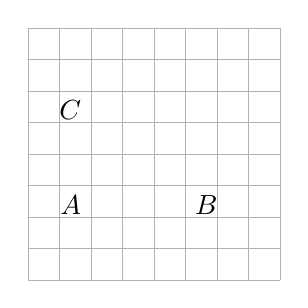
\begin{tikzpicture}[scale = 0.4]
            \draw[help lines, color=black!30] (0,0) grid (8,8);        
            \coordinate[label=below left:$A$] (A) at (2,3);
            \coordinate[label=below right:$B$] (B) at (5,3);
            \tkzDrawPoints[shape=cross out,size=3pt](A,B);
            %%%
            \coordinate[label=below left:{\red $C$}] (C) at (2,6);
            \tkzDrawPoints[shape=cross out,size=3pt,color=red](C);
        \end{tikzpicture}
        \item Construire $F$, l'image de $E$ par la rotation de centre $D$ et d'angle \ang{90}.\\
        \begin{tikzpicture}[scale = 0.4]
            \foreach \x in {0,1,...,8} {
                \foreach \y in {0,1,...,8} {
                    \fill[color=black] (\x,\y) circle (0.05);
                }
            }
            \coordinate[label=above left:$E$] (E) at (3,7);
            \coordinate[label=above right:$D$] (D) at (5,4);
            \tkzDrawPoints[shape=cross out,size=3pt](E,D);
            %%%
            \coordinate[label=above left:{\red $F$}] (F) at (2,2);
            \tkzDrawPoints[shape=cross out,size=3pt,color=red](F);
        \end{tikzpicture}
        \item Construire $K$, l'image de $H$ par la rotation de centre $G$ et d'angle \ang{60}.\\
        \begin{tikzpicture}[scale=0.5]
            \isometricPointGrid{7}{4}  
            \coordinate[label=above left:$H$] (H) at (4.5,6.055);
            \coordinate[label=above right:$G$] (G) at (6,3.46);
            \tkzDrawPoints[shape=cross out,size=3pt](H,G);
            %%%
            \coordinate[label=above left:{\red $K$}] (K) at (3,3.46);
            \tkzDrawPoints[shape=cross out,size=3pt,color=red](K);
        \end{tikzpicture}
    \end{enumerate}
    \Coupe
    \begin{enumerate}
        \setcounter{enumi}{3}
        \item Construire $N$, l'image de $M$ par la rotation de centre $L$ et d'angle \ang{120}.\\
        % \begin{tikzpicture}[scale=0.6]        
        %     \isometricGrid{5}{3}
        %     \coordinate[label=left:$M$] (M) at (2.5,0.865);
        %     \coordinate[label=left:$L$] (L) at (2,3.46);
        %     \tkzDrawPoints[shape=cross out,size=3pt](L,M);
        %     %%%
        %     \coordinate[label=above left:{\red $N$}] (N) at (4,5.19);
        %     \tkzDrawPoints[shape=cross out,size=3pt,color=red](N);
        % \end{tikzpicture} 
        \begin{Geometrie}[CoinHD={(3u,4u)}]
            % Pour changer la taille de la Grid
            coeff:=0.6;
            uni:=true;
            x.u:=coeff*cm;
            y.u:=coeff*(sqrt(3)/2)*cm;
            %%%            
            trace papiertriangle withcolor gris;
            pair L,M;
            L=pptri(0,4);
            M=pptri(2,1);
            marque_p:="croix";
            pointe(M,L);
            label.lft(btex $M$ etex,M);
            label.lft(btex $L$ etex,L);	
            %%%
            pair N;
            N=pptri(1,6);
            drawoptions(withcolor red);
            pointe(N);
            label.ulft(btex $N$ etex,N);	 
            drawoptions();
        \end{Geometrie}
    \end{enumerate}
\end{corrige}

